\documentclass{article}

\author{Teddy Krulewich}
\title{\vspace{-4em}HW6 ME5501 – Robotics and Unmanned Systems}

\usepackage{graphicx}
\graphicspath{ {images/} }

\usepackage{subcaption}
\usepackage{float}

\usepackage[utf8]{inputenc}
\usepackage{hyperref}
\usepackage{xcolor}
\definecolor{bg}{rgb}{0.95,0.95,0.95}
\usepackage{caption}
\usepackage{mdframed}

\usepackage{changepage}
\usepackage{enumitem}

\usepackage{titlesec}
\titleformat{\subsection}[runin]{}{}{}{}[]

\begin{document}
\maketitle

\section*{Source Code}

Full source code for all problems can be found on my GitHub repository:
\url{https://github.com/tkrulewich/teddy_krulewich_unmanned_systems/tree/main/teddy_krulewich_unmanned_systems/hw6/src/exam}


\section{Conceptual Questions}

\subsection*{\textbf{(a)}}

\textbf{Explain in what scenarios would RRT be the best choice (of the RRT, A*, Dijkstra’s
options)}

\bigskip
RRT is useful when the search space is very large, where other algorithms may take too long trying to fully explore the search space.


\subsection*{\textbf{(b)}}
\textbf{If you have a single starting point and 20 stops on your delivery run (traveling delivery
man). How many possible paths are there that visit each of the stops? Make sure to show
your work.}

\bigskip
Because you must always start at the same point, that stop is not considered. From that point there are 20 stops. The number of combinations of 20 items without replacement is: \\

\noindent $20!$ \\ = $20 \times 19 \times 18 \times 17 \times 16 \times 15 \times 14 \times 13 \times 12 \times 11 \times 10 \times 9 \times 8 \times 7 \times 6 \times 5 \times 4 \times 3 \times 2 \times 1 $
$= 2,432,902,008,176,640,000$

\subsection*{\textbf{(c)}}
\textbf{Describe how the genetic algorithm operates, and how it is applicable to the traveling salesman problem.}

\bigskip
A genetic algorithm is a search optimization technique that can rapidly find good solutions in problems where the solution space is very large. In the case of the TSP problem, the complexity and search space grows factorially, making large problem 
sizes infesible to solve with other methods by brute force methods.

The GA approaches this problem with the assumption that a good but suboptimal solution is likely to share features with better solutions, including the optimal.

To begin the GA generates a population of potential solutions, known as chromosomes. 
These chromosomes encode the solution as a sequence of genes. 
For example, in the case of the TSP, the genes could represent a sequence of cities or stops along the route.
A cost function is created to rank the fitness of each chromosome.
Then these chromosomes undergo a process of selection, crossover, and mutation, akin to natural selection, to produce a new generation of chromosomes.
The better chromosmes are selected to be parents, and combined with other parents. This creates offspring that share traits of both parents.
Mutations may then occur which may by chance improve the fitness of the chromosome.

\section{Trajectory Generating and Following Evader}

Your objective is to incorporate your Proportional Navigation pursuer turtlebot with an evader that
generates and follows an optimal path from a start to the goal. \textbf{You must provide a plot of each
bots’ path along with the desired trajectory generated for the evader.} You are not required to
include any obstacle avoidance into your pursuer path planning, but may find some small modifications
are required to successfully chase (and catch) the evader prior to the evader reaching the goal location
as well as make sure your evader does not collide with any obstacles. \textbf{In addition to the plot(s),
provide the code used for the problem, and provide any comments/discussions necessary
to interpret your results and describe any modifications you had to make in order to be
successful.}

\bigskip
\noindent Launch File: two turtlebot3 test.launch \\
World File: umkc test.world \\
Obstacle List: (5, 0),(5, 1),(5, 2),(5, 3),(5, 4),(0, 5),(1, 4),(2, 3),(3, 2),(3, 3) \\
Evader Parameters: Name - turtlebot1, Start - (2.0, 1.0), Goal - (7.0, 2.0), Max Speed - 0.15m/s \\
Pursuer Parameters: Name - turtlebot2, Start - (0.0, 0.0), Maximum Speed - 0.2m/s \\ 
Algorithms: Pursuer - Proportional Navigation, Evader - Dijkstra’s Algorithm \\

\bigskip
\noindent  All of the code can be found at: \\
\url{https://github.com/tkrulewich/teddy_krulewich_unmanned_systems/blob/main/teddy_krulewich_unmanned_systems/exam/src/exam/exam/question2.py}

\bigskip
\noindent The code for the pursuer can be found here: \\
\url{https://github.com/tkrulewich/teddy_krulewich_unmanned_systems/blob/main/teddy_krulewich_unmanned_systems/exam/src/exam/exam/submodules/PursuerTurtleBot.py}

\bigskip
\noindent A plot of the pursuer and evader trajectories can be seen below:

\begin{figure}[h]
\centering
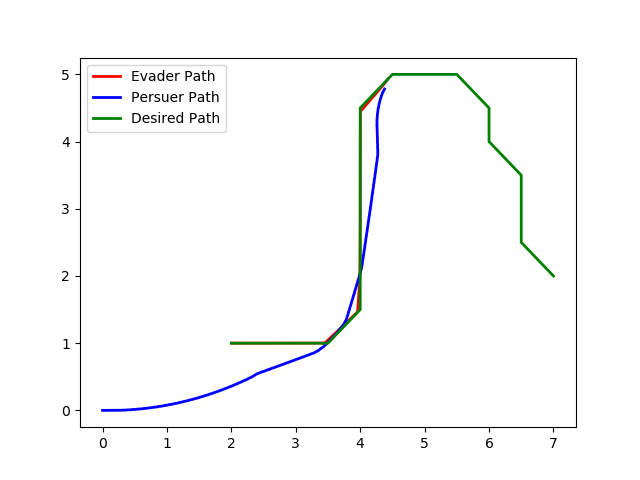
\includegraphics[width=0.95\textwidth]{images/intercept.png}
\caption*{Pursuer and Evader Trajectories}
\end{figure}

The default settings for the turtlebot and ros seem to be incompatible with proportional navigation. I was able to get it to work, but I had to modify the turtlebot source code and increase the update frequency of the lidar as well as the resolution.

After modifying my turtle bots I ran into a different problem. The pursuer was running into walls. I was able to combat this some of the time by telling the turtlebot to only target things that didn't have a lot of consecutive. In other words, the pursuer the closest point it detects as long as that point is not close to many other points.

\section{Traveling Salesman Problem with A*}

Your objective is to use the \textit{A* Algorithm} to navigate through the modified maze (obstacle list posted
below) to deliver five packages. You must start at (0,0) and visit each of the delivery points. Provide a
plot showing the obstacles, A* paths, and delivery locations. Provide the total travel distance of your
solution. How does this compare with the other possible paths (how good is the solution, are there other
paths that have much higher travel costs)? Turn in a copy of your working code.

\pagebreak
\bigskip
\noindent\textbf{Grid Info:} Xmin = 0, Xmax = 15, Ymin = 0, Ymax = 15, Grid Size = 0.5, Robot Radius = 0.5 \\
\textbf{Delivery Points:} (9,4), (4,4), (1,9), (9,7), (6,14) \\
\textbf{Obstacle List:} (2,2), (2,3), (2,4), (2,5), (0,5), (1,5), (2,5), (3,5), (4,5), (5,5), (8,2), (9,2), (10,2), (11,2),
(12,2), (13,3), (8,4), (8,5), (8,6), (8,7), (8,8), (8,9), (8,7), (2,7), (3,7), (4,7), (5,7), (6,7), (7,6), (9,6),
(10,6), (11,6), (12,6), (15,8), (2,9), (2,10, (2,11), (2,12), (2,13), (5,9), (5,10), (5,11), (5,12), (5,13),
(5,14), (5,15), (6,12,0.5), (7,12), (8,12), (9,12), (10,12), (11,12), (12,8), (12,9), (12,10), (12,11), (12,12) \\

\noindent \textbf{Note: See obstacle problem2.py on Canvas for obstacle list typed in already. This should
save you from any copy-paste errors.}

\bigskip
\noindent The code can be found here: \\
\url{https://github.com/tkrulewich/teddy_krulewich_unmanned_systems/blob/main/teddy_krulewich_unmanned_systems/exam/src/exam/exam/question3.py}

\bigskip
\noindent Since there are 5 cities, there are 5! or 120 different possible paths. I'm not going to show all of them, but here are a few:


\bigskip
\noindent The best path found by brute force was \\
Path: (0, 0), (4, 4), (9, 4), (1, 9), (9, 7), (6, 14) \\
Distance: 54.970562748477136 and a plot is seen below:

\begin{figure}[H]
\centering
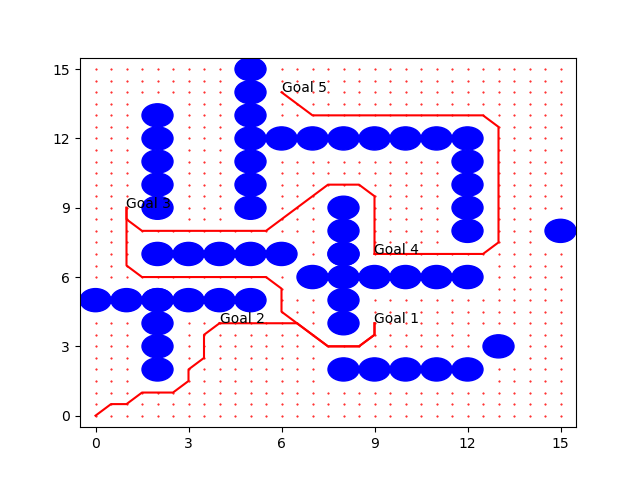
\includegraphics[width=0.75\textwidth]{images/question3.png}
\caption*{5 City TSP Path With Obstacles}
\end{figure}

\section{Super TSP - Brute Force}

You have a map very similar to Problem 2 (just a few obstacles removed),
with many more waypoints that must be visited. The vehicle \textbf{must} start from the first delivery point
(1,1). Use your A*-based TSP code to identify the best path. Plot identical to Problem 2. Please note
this will take 10 minutes up to 60 minutes to compute (based on your computer performance). It is
recommended to use the tqdm package to keep track of timing. Simply put “from tqdm import tqdm”
at the top, and in your big for loop put “for i in tqdm(range(0,len(perm list))):” \\

\bigskip
\noindent\textbf{Grid Info:} Xmin = 0, Xmax = 15, Ymin = 0, Ymax = 15, Grid Size = 0.5, Robot Radius = 0.5 \\
\textbf{Delivery Points:} (1,1), (9,7), (1,9), (4,4), (9,4), (6,14), (3,11), (14,1), (1,14), (14,14), (7,10)

\bigskip
\noindent\textbf{Note: See obstacle problem3.py on Canvas for obstacle list typed in already. This should
save you from any copy-paste errors.}

\bigskip
\noindent Provide the computation time, and the minimal total travel cost

\bigskip
The code can be found here: \\
\url{https://github.com/tkrulewich/teddy_krulewich_unmanned_systems/blob/main/teddy_krulewich_unmanned_systems/exam/src/exam/exam/question4.py}
\\

\noindent The best path found by brute force was \\

\noindent Path: (0, 0), (1, 1), (4, 4), (14, 1), (9, 4), (9, 7), (7, 10), (3, 11), (1, 9), (1, 14), (6, 14), (14, 14) \\ \\
Distance: 75.55634918610404 \\
Time taken: 54.20994830131531 seconds

\begin{figure}[H]
\centering
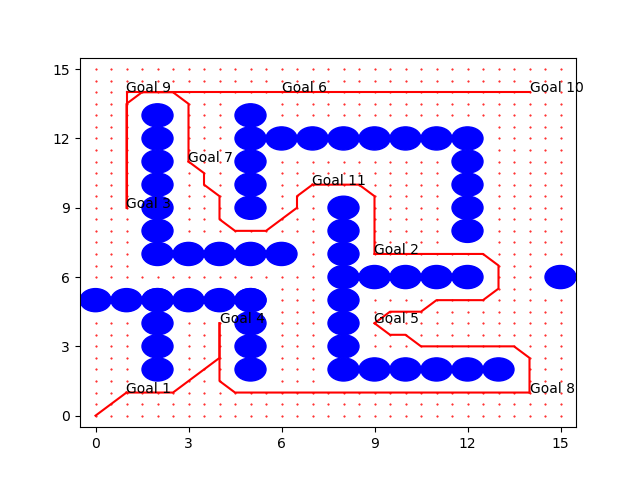
\includegraphics[width=0.75\textwidth]{images/question4.png}
\caption*{11 City TSP Path With Obstacles}
\end{figure}

\section{Super TSP - Genetic Algorithm}

Use the same map/obstacles as Problem 3. You must use a
Genetic Algorithm to solve the TSP. It is recommended to use/adapt the code provided on Canvas. It
is recommended to comment the code (as you need to understand the basics of how it is working to
make the changes). There are several ways to approach this problem, but keep in mind you must start
at the first ”city” or waypoint. The code currently just provides the best path (can start at any city).
It is recommended to remove the first city from the list, and add it in whenever computing the current
path cost (or fitness). This is an easy solution that doesn’t require a lot of modifications in the code.

\bigskip
\noindent Use a population size of 500, with 2,000 generations. \\
Provide the computation time, and best path cost. \\
Provide a plot of the obstacles with path (identical to previous problems).

\bigskip
\noindent The code can be found here: \\
\url{https://github.com/tkrulewich/teddy_krulewich_unmanned_systems/blob/main/teddy_krulewich_unmanned_systems/exam/src/exam/exam/question5.py}

\bigskip
\noindent I implemented my own GA for this problem, because I don't read directions well.
My GA found the same path as the brute force method, but much more quickly.

\bigskip
\noindent Below is the output of running the GA. Output is updated every time a better path is found.
\begin{figure}[H]
\centering
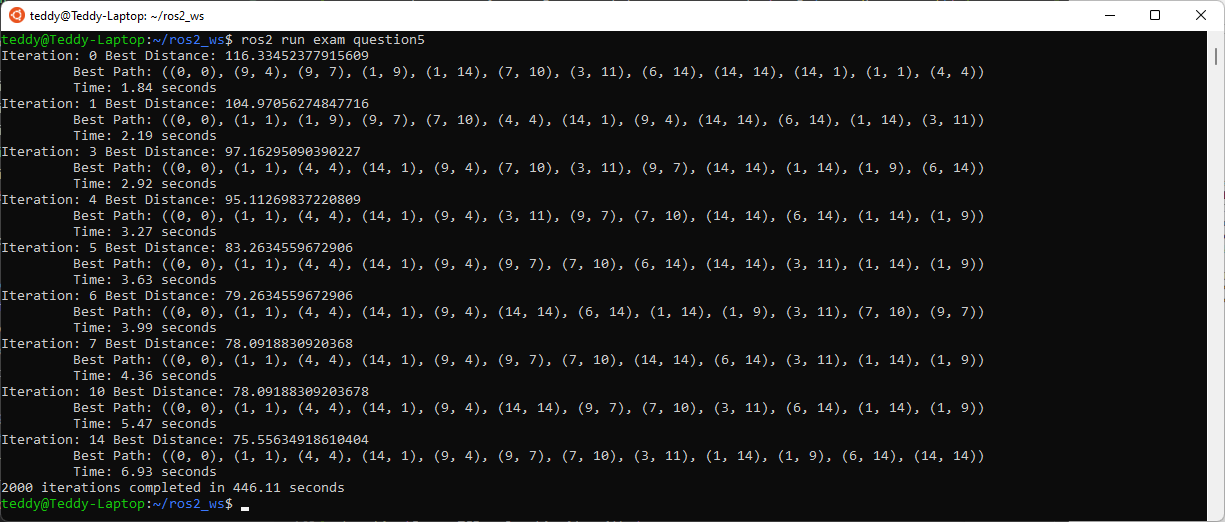
\includegraphics[width=1.0\textwidth]{images/question5-console.png}
\caption*{11 City TSP Path With Obstacles}
\end{figure}

As seen above the optimal solution was actually found by generation 14 at 6.93 seconds, much faster than brute force. This did vary however, at times taking a bit longer.

Running the GA to completion took longer than the brute force for this problem size, but it had actually converged upon a solution much sooner. 2000 generations took a total of 446.11 seconds.

\end{document}